\documentclass{egee}
\usepackage{comment,alltt}

\def\LB{L\&B}

\title{gLite Job Provenance service User's Guide}
\author{CESNET EGEE JRA1 team}
\DocIdentifier{EGEE-JRA1-??}
\Date{\today}
\Activity{JRA1: Middleware Engineering and Integration}
\DocStatus{DRAFT}
\Dissemination{PUBLIC}
\DocumentLink{}

\Abstract{

  Job Provenance (JP) service provides long-term storage of data
  related to job live in a Grid. JP provides a query interface
  allowing to perform data-mining. The possibility to annotate jobs
  stored in JP is also provided.

  There is a overview of the service architecture followed by main JP
  use case scenarios in this document. Technical reference
  documentation for both JP user and JP administrator is included in
  this document too.  This user's guide also contains release notes
  describing current JP implementation.

  For actual version of this document see
  \texttt{http://egee.cesnet.cz/en/JRA1/} web page.
}

\def\todo#1{\textbf{TODO:} #1}

\begin{document}

%\begin{center}
{\bf Delivery Slip}
\end{center}
\begin{tabularx}{\textwidth}{|l|l|l|X|X|}
\hline
           & {\bf Name} & {\bf Partner} & {\bf Date} & {\bf Signature} \\
\hline
{\bf From} &                  &  & & \\
\hline
{\bf Reviewed by} & &  & & \\

\hline
{\bf Approved by} & & & & \\
\hline
\end{tabularx}

\begin{center}
{\bf Document Change Log}
\end{center}

\begin{tabularx}{\textwidth}{|l|l|X|X|}
\hline
{\bf Issue } & {\bf Date  } & {\bf Comment } & {\bf Author  } \\   \hline

\hline
\end{tabularx}

\begin{center}
{\bf Document Change Record}
\end{center}

\begin{tabularx}{\textwidth}{|l|l|X|}
\hline
{\bf Issue } & {\bf Item  } & {\bf Reason for Change } \\   \hline

\hline
\end{tabularx}

%
% Official text received on October 6, 2004
%
\vfill{\bf Copyright }\copyright{\bf Members of the EGEE Collaboration. 2004. 
See http://eu-egee.org/partners for details on the copyright holders. 

EGEE (``Enabling Grids for E-science in Europe'') is a project funded by
the European Union.  For more information on the project, its partners
and contributors please see http://www.eu-egee.org.

You are permitted to copy and distribute verbatim copies of this
document containing this copyright notice, but modifying this document
is not allowed. You are permitted to copy this document in whole or in
part into other documents if you attach the following reference to the
copied elements: ``Copyright }\copyright{\bf 2004. Members of the EGEE
Collaboration. http://www.eu-egee.org''

The information contained in this document represents the views of
EGEE as of the date they are published. EGEE does not guarantee that
any information contained herein is error-free, or up to date.

EGEE MAKES NO WARRANTIES, EXPRESS, IMPLIED, OR STATUTORY, BY
PUBLISHING THIS DOCUMENT.}


\clearpage

%\newpage
\tableofcontents
\newpage

\section{Job Provenance service overview}
The information about jobs submitted to gLite Workload Management
System is collected by the Logging and Bookkeeping (LB) service.
LB tracks jobs in terms of events and processes them in
a~real time to give overall view on the actual job state. The user may
query the bookkeeping server to obtain either the raw events or the
computed job state, she may also register for receiving notifications
on particular job state changes.

While the LB is intended to keep track of jobs during its lifetime, it
is not supposed to be used for long term archival of such data. The
Job Provenance (JP) service is designed to provide long-term storage
of all data related to job life and allow the end user to perform
data-mining in this data.
The JP is supposed to provide the permanent storage of
the job related information as stored within the \LB, to couple it with
the input sandboxes and other system oriented information necessary to
reproduce the environment where a~particular job run.

\subsection{Gathering data into Job Provenance}
Fig.~\ref{fig:psinter} depicts basic gLite middleware components and
their interaction with the Job Provenance.

\begin{figure}[htpb]
  \centering
  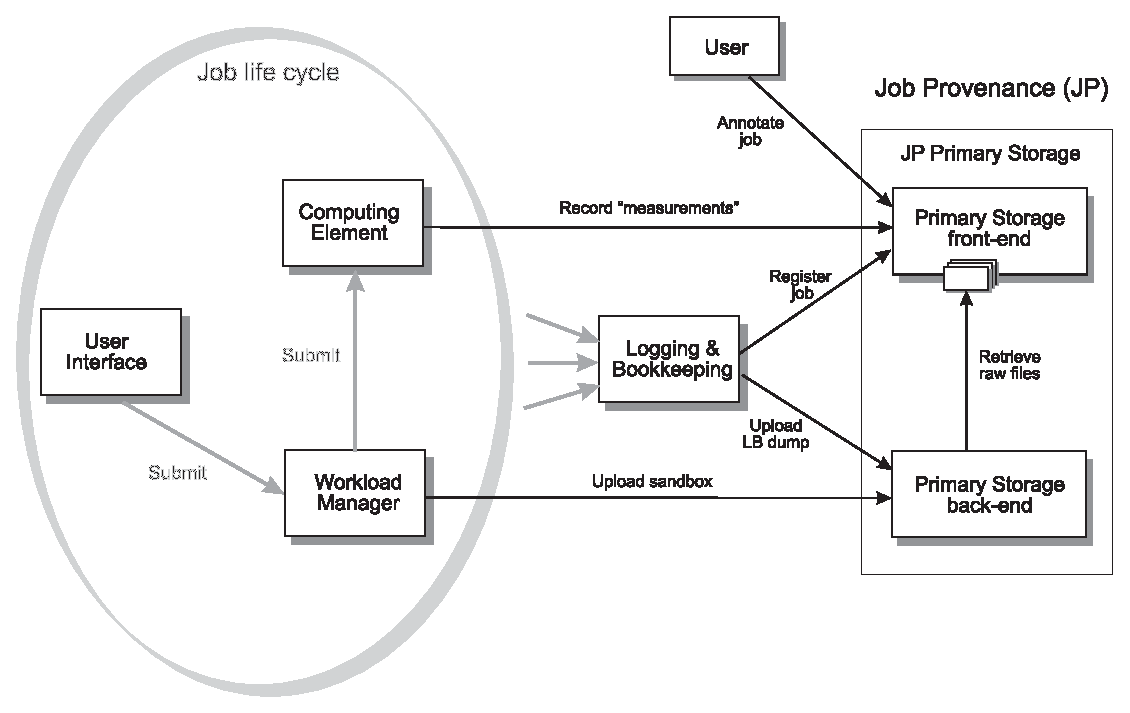
\includegraphics[scale=0.7]{JP-interactions}
  \caption{Data flow into gLite Job Provenance}
  \label{fig:psinter}
\end{figure}

JP is formed of two classes of services: permanent \emph{Primary
Storage} (JPPS) accepts and stores job data while possibly volatile
and configurable \emph{Index Servers} (JPIS) provide an optimized
querying and data-mining interface to the end-users.  The only direct
data retrieval scenario supported by JPPS is the case when user know exact ID
of jobs in the interest.

\subsection{Getting data from Job Provenance}

The role of \emph{Index Servers} (JPIS) is processing and re-arranging the data
from Primary Storage(s) into a~form suitable for frequent and complex user
queries. A user query part of JP is shown in Fig.~\ref{fig:query}.

\begin{figure}[htpb]
  \centering
  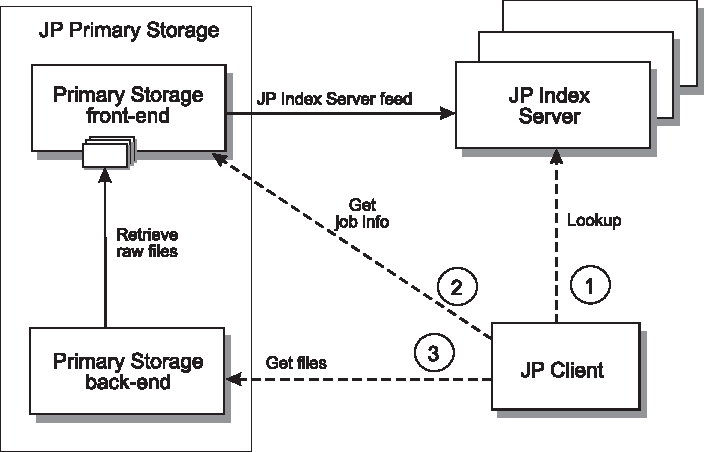
\includegraphics[scale=0.8]{JP-query}
  \caption{Index Server interactions}
  \label{fig:query}
\end{figure}

Index Servers are created, configured, and populated semi-dynamically
according to particular user community needs.  It is responsibility of
its administrator to setup the JPIS with appropriate configuration. There
is no prescribed relationship between Primary Storage and Index Server
installations.  An Index Server may retrieve data from multiple
Primary Storages and vice versa.

The interface exposed by JPIS to the end user is described in the
chapter~\ref{reference}. Command line interface tool for end-user
interface to the JPIS is described in the chapter~\ref{CLI}.  See the
next chapter (use cases) for futher description of JP to user
interactions.

\section{Job Provenance use cases}

\subsection{Prerequisities}

\subsubsection{LB/JP relationship}
When JP deployed, any job in a terminal state will disappear from LB
after preconfigured timeout (one week for example). If a user wants
any information about such a job before this timeout (or before it
reach a terminal state) he must use the LB service (please refer to LB
user's guide). After that timeout he must use the JP service.

For LB configuration please see gLite installation guide. For a
technical description of LB-JP interactions please see
\texttt{http://egee.cesnet.cz/en/JRA1/LB-JP-interaction-guide.pdf}.

\subsubsection{JP service location}
To call JP you need to know JP services address. There are two services:
\begin{itemize}
\item JP primary storage (JPPS)\\
  From JP design point of view there are only few PS in the
  grid. Expected implementation is that these JPPS locations
  are preconfigured in a UI instance while one of them is configured as
  default JPPS.
\item JP index server (JPIS)\\
  Each index server is build (configured and started) by site/VO/user
  group administrator (or even "senior user") based on given
  community needs (expected queries and its optimization). So in
  principle the index server location for a given query is to be
  provided by the user. We expect that the UI instance will provide
  mechanism allowing selection from preconfigured JPIS servers list.
\end{itemize}

\subsection{JP use case 1 -- get job info}

The scenario:
\begin{itemize}
\item The user wants information about a particular job. He knows a
  job id. Job isn't longer in the LB. Procedure: Ask the JPPS to get all
  or selected attributes of job.
\end{itemize}

The implementation:
\begin{itemize}
 \item Let a user to specify attributes to be returned. See section
  \ref{attributes}.
 \item Call GetJobAttributes operation of a JPPS and display the values
  returned.
\end{itemize}

Examples and hints:
\begin{itemize}
 \item \texttt{org.glite.jp.primary/examples/jpps-test.c}\\
  This utility is used for all JPPS operations. Some hints how to use it
  can be find in the test plan document.
\end{itemize}

\subsection{JP use case 2 -- get job files}

The scenario:
\begin{itemize}
 \item The user knows a job id, job is in a terminal state. The user wants
  all files (LB event dump, sandbox) stored by JP for futher processing.
\end{itemize}

The implementation:
\begin{itemize}
 \item Call GetJobFiles operation of a JPPS. You will get a list of URLs
  which can be used to download the files.
\end{itemize}

Examples and hints:
\begin{itemize}
 \item The same as use case 1.
\end{itemize}

\subsection{JP use case 3 -- job lookup}

The scenario:
\begin{itemize}
 \item The user is looking for jobs with specific properties. In this case
  (no job id known) a JPIS must be used. There are the same query interface
  provided by any JPIS but if a particular query can be answered by
  the given JPIS depends on its configuration (configuration
  determines which attributes are uploaded by PS to IS, and which of
  them are indexed).
 \item The user should know the proper JPIS to use for its particular
  needs.
 \item The scenario can continue by the JP use cases number 1 and 2 described
  above (JPIS answer will contain job ids and identification of JPPSs
  to ask for all available JP data about the jobs).
\end{itemize}

The implementation:
\begin{itemize}
 \item The user will select a JPIS and provide query. The JPIS operation
  QueryJobs is called and list of jobs matching the query is returned.
\end{itemize}

Examples and hints:
\begin{itemize}
 \item JPIS CLI tool\\
   org.glite.jp.index/examples/jpis-client.c

 \item example in org.glite.jp.index/examples/jpis-test.c (starting
   from line 161)
\end{itemize}

\subsection{JP use case 4 -- job annotation}

The scenario:
\begin{itemize}
 \item The user wants to add a user tag (annotation) to a job. He must know
  the job id(s) (or use the JP use case number 3 to find it).
\end{itemize}

The implementation:
\begin{itemize}
 \item Call RecordTag operation of JPPS for the job(s) to add requested
  user tag.
\end{itemize}

Examples and hints:
\begin{itemize}
 \item The same as use case 1.
\end{itemize}


\subsection{Job attributes}
\label{attributes}
Job attributes are referenced by its names. Each attribute belongs to
one namespace (represented by a prefix in the attribute name).

A namespace is defined by a service (currently we have one for LB and
one for JP) providing its data to the JP or a user group/experiment
who wants to attach its own data to the job.

It is expected that UI have preconfigured list of available namespaces
and XML schema for each namespace (the schema can be automatically
retrieved based on the namespace name). A list of available attributes
is generated from these schemas when user have to select attributes to
be retrieved from JP.

\begin{itemize}
 \item The namespaces (schema is available at the URL representing namespace):\\
  http://egee.cesnet.cz/en/Schema/LB/Attributes\\
  http://egee.cesnet.cz/en/Schema/JP/System   <<<<<<<(NOT YET)\\
 \item There are header files with known names of attributes generated from
  these schema files in our build procedure:\\
  org.glite.lb.server/build/jp\_job\_attrs.h\\
  org.glite.jp.common/interface/known\_attr.h  <<<<<<<\\
\end{itemize}

\subsection{Authentication and authorization}
All the calls must be authenticated by user credentials. In the
current JP release only implicit ACLs are available -- the job
information is available for job owner only.


\section{Release notes}
\todo{TBD}

\section{References}

%\subsection{Role of the JP administrator}
% Podle Ljochy sem nepat��. Podle mne mus� u�ivatel v�d�t kdy a s ��m
% otravovat administratora (zejm�na IS).

\begin{itemize}
 \item In general, the page \texttt{http://egee.cesnet.cz/en/JRA1} should
  contain actual versions of JP documentation.

\item Interfaces (WS):
 \begin{itemize}
  \item In source code tree the WSDLs are located in these files:\\
   \texttt{org.glite.jp.ws-interface/src/JobProvenanceIS.xml,\\
   org.glite.jp.ws-interface/src/JobProvenancePS.xml,\\
   org.glite.jp.ws-interface/src/JobProvenanceTypes.xml
   } 
 \end{itemize}
 \item Namespaces of attributes -- see section \ref{attributes}
 \item Job provenance test plan\\
 \texttt{http://egee.cesnet.cz/en/JRA1/testplan.pdf}
\end{itemize}

\subsection{Command line interface (CLI)}
\label{CLI}
{
\newcommand{\dbz}{}
\newcommand{\docbooktolatexpipe}{\ensuremath{|}}
\newskip\docbooktolatexoldparskip
\input glite-jpis-client
}

\subsection{JP web-service interface reference}
\label{reference}

{
\parindent0pt
\def\chapter#1{}
\def\section#1{\subsubsection{#1}}
\def\subsection#1{\par\medskip\textbf{#1}\par}

\let\odesc=\description
\let\oedesc=\enddescription
\renewenvironment{description}{\odesc\itemindent=1em
\listparindent=2em
}{\oedesc}
%\renewenvironment{description}{\list{}{\labelwidth 5cm\leftmargin 5cm}}
%{\endlist}

\let\null=\relax
\input jpws
}



\end{document}
